\documentclass[a4paper,12pt,french]{article}
%Déclaration des packages

\usepackage[latin1,utf8]{inputenc}  
\usepackage{ucs}
\usepackage{url}
\usepackage[babel=true]{csquotes}
\usepackage{amsfonts,amsmath,amsthm}
\usepackage[french]{babel}
\usepackage{graphicx}
\usepackage{tikz}
\usepackage{lscape}
\usepackage{chngpage}
\usepackage{pifont}
\usepackage{listingsutf8}
\usepackage{listings}
\usepackage{color}
\usepackage[T1]{fontenc}
\usepackage{hyperref}
\usepackage{enumitem}
\newcommand{\ul}{\underline}

\lstset{inputencoding=utf8/latin1}
\lstnewenvironment{code}[1][]{  
 \lstset{
  basicstyle=\largel,
  columns=flexible,
  basicstyle=\ttfamily,
  language=Python,  % On choisit le language qui sera utilise dans cet environnement
  morekeywords={input},
  keywordstyle=\color{blue},  % On choisit la couleur des mots cles (def, while, if, for, try et tous les autres) de python
  commentstyle=\color{red!90},  % On choisit la couleur des commentaires
  breaklines,
  breakindent=1em, % On regle l'espacement pour l'indentation
  xleftmargin=0.2em, % On regle la marge de gauche (a l'interieur de la "boite" de code)
  xrightmargin=0.2em, % On choisit la marge de droite
  frame=single,
  rulecolor=\color{orange},
  backgroundcolor=\color{yellow!40}, % Le fond est a 30% de couleur jaune
  #1
 }
}{}

\setlength\fboxrule{1pt}
\setlength{\parskip}{1em}

% Début du document
\begin{document}
\title{Rapport Projet de Synthèse}
\author{Marius AMBAYRAC et Andrés Garcia}
\date{2018}
\maketitle
\clearpage
\tableofcontents
\clearpage

\section{Introduction}
% Idée : On explique ce qu'est le codage,
% Introduire à la fois le codage canal et le codage de source puis
% expliquer que l'on va s'intéresser en priorité au codage de source

Que ce soit dans l’envoi d’un fac-similé, le stockage de données comme peut être une image digitale ou le téléchargement d’un fichier MP3, les outils numériques et plus généralement, la théorie de l’information est devenue de nos jours la base fondamentale des communications à distance. Avec la digitalisation des contenus, le gain de vitesse en termes de calcul informatique des dernières décennies et la démocratisation des technologies, notre société est capable aujourd’hui de transmettre de l’information d’un coin du monde à l’autre en quelques secondes à travers une multitude de moyens, permettant ainsi de travailler en réseau et d’établir des liens qui autrement seraient impossibles. Toutefois, à chaque seconde cette société génère d’énormes flux d’informations et les technologies de la communication ont du savoir se réinventer. Pour résoudre ce problème, le codage est apparu.

Le codage correspond simplement à la transition d’une représentation de données selon un système de règles vers un autre différent. Parmi tous les codages, on différencie notamment deux types : le codage de canal, qui vise à utiliser une représentation plus redondante résistante aux erreurs de transmission tels que le bruit ; et puis le codage de source, codage sur lequel nous nous intéresserons sur ce travail et qui permet de compresser ces données (avec ou sans perte d’information). Les deux sont donc complémentaires et Shannon démontra que, dans certains cas, cette distinction opérationnelle est asymptotiquement optimale. Cependant, avant de continuer, il faudrait se poser plusieurs questions : Qu’est-ce qu’on comprend par « se communiquer », quels sont ces technologies existantes dont on en parle et quels sont les problèmes et limitations que nous retrouvons sur les modèles ?
Cette étude est divisée en deux parties : dans la première, on comprendra et analysera la fondation théorique qu’existe derrière les moyens de communication actuels pour, dans un deuxième temps, approfondir dans l’implémentation sur différentes sources d’une méthode concrète de codage de source : le Codage entropique de Huffman à longueur variable.

\section{Partie Théorique}
% Développer les différents aspects du codage de source
Dans la suite de cette partie, nous établirons la base théorique qui permet le postérieur développement pratique à travers les notions des bases qui expliquent la caractérisation d’une communication efficace et puis ses conséquences moins évidentes.


	\subsection{Définitions essentielles}
	% On introduit ici les définitions de base, les autres seront introduites au fur et à mesure, plus tard
	
	La première notion fondamentale à prendre conscience est le Paradigme de Shannon. Etudié par Claude E. Shannon et Warren Weaver en 1949, ce modèle s’agit d’un scénario conçu d’une façon schématique pour représenter \textit{la transmission d'un message} à travers un système de communication.
	
	\begin{center} 
    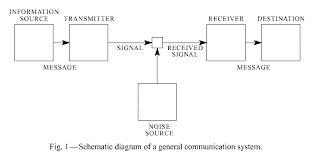
\includegraphics[scale=1.5]{shannon.png}
    \label{Schéma de Shannon} 
    \end{center}
	
	Sur celui-ci, la transmission du message démarre par la source, siège d’évènements aléatoires à l’origine du message émis et caractérisée par son \textit{entropie} (qui consiste à une quantité \textit{moyenne} d’information produite et est relié au concept d’\textit{incertitude}. Ensuite se déroule le codage en source (élimine de la redondance et réduit la taille du message) et le codage canal sur le canal (qui transmet et dégrade le message) caractérisée par une \textit{capacité}. Finalement les phases de décodages correspondantes (opérations réciproques pour restituer le message) avant d’arriver au destinataire.
    
    Cette théorie est une théorie probabiliste et pour pouvoir continuer, il est nécessaire de citer quelques outils de base qui serviront à introduire la notion d’entropie.
    
    La réalisation d’un évènement (comme l’est la réception d’un message déterminé) nous procure de l’information seulement si son contenu nous était inconnu à l’avance. En effet, et dans la même logique, on peut dire que plus un évènement est rare (et donc plus sa probabilité de réalisation est faible), plus grande est la surprise ressentie lorsqu’il apparaît, i.e. l’information que nous apprenons une fois on le détecte. Pour pouvoir mesurer cette \textit{incertitude} de l’évènement, Shannon proposa la formule suivante :

	\begin{equation}
	    h(E) = log(\frac{1}{P(E)})
	\end{equation}
	
	De la même façon, nous pouvons aussi réfléchir à l’idée d’incertitude d’un évènement pour une probabilité conditionnelle sachant que B a été déjà réalisé :
	
	\begin{equation}
	    h(E/B) = log(\frac{1}{P(E/B)})
	\end{equation}
	
	Les études de Shannon prennent compte aussi sur la fondation de cette théorie à l’idée primordiale, celle d’information. Sur la base de l’incertitude, on dit que l’information que B apporte sur l’évènement E correspond à la différence des deux incertitudes précédentes :
	
	\begin{equation}
	    I(B,E) = h(E) - h(E/B) = h(B) - h(B/E)
	\end{equation}
	
	D’autre part, en se limitant aux sources discrètes (la plupart d’elles peuvent être considérées ainsi), on peut les décrire comme des dispositifs susceptibles de fournir de façon aléatoire des symboles issus d’un ensemble fini qu’on appellera \textit{alphabet} (« A ») à m \textit{éléments}. De cette façon, les données émises par une source U pourront être modélisées par une suite de variables aléatoires $U_{1}$, $U_{2}$, … à valeurs dans A suivant une loi probabilistique déterminée et chaque symbole sortant de cette source à des instants donnés correspondront à une réalisation de la variable aléatoire $U_{k}$ correspondante. De plus, la source $U$ sera dite une source m-aire.
    
    Ensuite, nous parlons de source stationnaire lorsque les propriétés probabilistes de la réalisation de ces évènements sont stables dans le temps, i.e. les différents $U_{k}$ ont la même loi de probabilité. Parallèlement, on dit que la source a une mémoire d’ordre n lorsque la loi de probabilité du $U_{k+1}$ dépendent des n variables $U_{k}$, $U_{k-1}$, …, $U_{k-n}$ antérieures et c’est pour le cas particulier de n = 1 que nous travaillons sur une source markovienne.
    
    Néanmoins, comme on vient de dire, une source U peut être représentée par une variable aléatoire qui à son tour, se réalise sur un nombre fini de potentiels évènements et c’est ici où on réalise le parallélisme : tous les concepts antérieurs peuvent être étendus d’un évènement en particulier à toute une source et plus précisément, la moyenne pondérée des incertitudes des réalisations de la variable aléatoire U est appelée \textit{entropie} H(X) et est calculée ainsi :

    \begin{equation}
    H(X) = \sum_{i=1}^{n} p_{i} * log (\frac{1}{p_{i}}) = - \sum_{i=1}^{n} {p_{i} * log (p_{i}}) 
    \end{equation}

    Et de même, l’entropie conditionnelle de Xk sachant Xk-1 (comme arrive à une source markovienne) :
    
    \begin{equation}
    H(X_{k}/X_{k-1}) = - \sum_{j=1}^{n} P(X_{k-1} = x_{j}) * H(X_{k}/X_{k-1} = x_{j}) 
    \end{equation}

    Pour terminer, si on élargit la définition d’information pour une variable aléatoire X sur Y :
    
    \begin{equation}
    I (X,Y) = h(X) - h(X/Y) = h(Y) - h(Y/X)
    \end{equation}
    
    qui après développement correspond à :
    
    \begin{equation}
    I(X,Y) = E  \left[log \frac{P(X,Y)}{P(X)P(Y)}  \right] \geq 0
    \end{equation}
    
    avec l’égalité lorsque X et Y sont indépendants (le cas des sources sans mémoire). On peut donc conclure qu’une source à mémoire non nulle aura toujours moins d’entropie (c’est-à-dire, sera plus prévisible) qu’une sans mémoire. Ceci est facilement observable sur une source markovienne : le fait d’être sur un certain « état » permet de limiter les états suivants possibles.

	\subsection{Inégalité de Kraft-McMillan}
	
	Une fois que nous avons défini correctement ce qu’est la source, nous pouvons enfin décrire la démarche du codage source. 
    
    Du point de vue formel, un codage source C pour une variable aléatoire X modélisant une source correspond à un \textit{data mapping} entre les évènements de l’univers X (support de X) à D, l’ensemble des vecteurs finis composés de symboles d’un alphabet k-aire A. Chacun de ces vecteurs sera appelé mot-code de xi selon C. De plus, on parle de codage \textit{non-singulier} lorsque la transformation C est injective :

     \begin{equation}
    x_{i} \neq x_{j} \rightarrow C(x_{i}) = C(x_{j})
    \end{equation}
    
    et aussi sera de \textit{longueur fixe} si tous les mots-code image de X ont la même taille d’éléments structurels fondamentaux (pour le codage binaire, on décrit ainsi les \textit{bits}). Grâce à ce type d’applications, nous sommes capables de traduire n’importe quelle donnée d’un langage à un autre juste en précisant quels sont les liaisons entre les éléments des deux espaces. En revanche, ce fait succinct pas mal d’interrogatifs : est-ce que n’importe quel ensemble de liaisons est valable ? Et parmi ceux qui le sont, est-ce que tous sont aussi efficaces que les autres ou au contraire, nous pouvons converger sur une optimalité, notamment en termes de gain en longueur de la nouvelle représentation de la donnée ?
	
	\subsection{Bornes sur la longueur moyenne attendue d'un code}
	
	\subsection{Optimalité du Codage de Huffmann}
	
	\subsection{Limitations du Codage de Huffmann}
	
\section{Partie pratique}

	\subsection{Source binaire sans mémoire}
	
	\subsection{Source binaire Markovienne}
	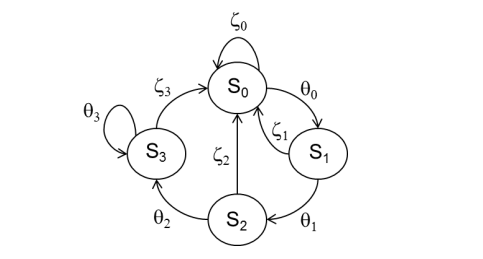
\includegraphics[scale=1]{SourceAvecMemoire.png}
	
\section{Bibliographie}
 	
\section{Annexe}	
	\subsection{Petites Fonctions}
		\subsubsection{Calcul de l'entropie}
		\begin{code}
		def entropie(tab_proba):
    '''Cette fonction calcule l'entropie du tableau de probabilité fourni en entrée sous la forme de tuple (frequence, motif)'''
    somme = 0
    for (pi,elm) in tab_proba:
        somme += pi*log(pi,2)
    return -somme
		\end{code}
		\subsubsection{Longueur moyenne d'un codage}
		\begin{code}
		def longueur_moyenne(source,codage):
    '''Cette fonction calcule la longueur moyenne d'un codage. Elle prend en entrée une liste de tuple (frequence,motif) et une autre liste de tuple (code, motif).'''
    long = 0
    for (freq,motif) in source:
        for (code,motifBis) in codage :
            if motif==motifBis :
                long += len(code)*freq
    return long
    \end{code}
	\subsection{Codage de Hamming}
	\begin{code}
	def Huffman(tab_proba):
    """Cette fonction prend en entrée une liste de tuple (frequence,motif)
    et retourne une liste de tuple (code, motif)"""
    m = len(tab_proba)
    C = [("0","Initial")]*m                                                                #C est le tableau de tuple que l'on renverra, il est composé de (code, motifACoder)
    if m == 2 :                                                                            #Cas de base de notre algorithme récursif
        C[0],C[1] = ("0",tab_proba[0][1]),("1",tab_proba[1][1])
    else :
        tab_proba.sort(reverse = True)                                                     #On trie la liste des proba dans le sens décroissant
        temp = Huffman(tab_proba[0:-2] + [(tab_proba[-2][0]+tab_proba[-1][0],"new")])      #On applique le procédé sur une liste de taille m-1
        indice = recup(temp,"new")                                                         
        #On regarde ou l'élément "spécial" s'est positionné suite au tri
        temp.append(temp[indice])
        temp.pop(indice)                                                                    #On l'enlève pour le repositionner à la fin de la liste
        for i in range(m-2):                                                                #On récupère les codes pour les m-2 premiers motifs
            C[i] = temp[i]
        C[m-2] = (temp[-1][0]+"0",tab_proba[-2][1])                                         #On crée les codes pour les 2 derniers motifs
        C[m-1] = (temp[-1][0] + "1",tab_proba[-1][1])
    return C
	\end{code}
\end{document}